\ifdefined\pdfinfoomitdate\pdfinfoomitdate=1\fi
\ifdefined\pdftrailerid\pdftrailerid{}\fi
\ifdefined\pdfsuppressptexinfo\pdfsuppressptexinfo=15\fi
\documentclass[11pt]{article}
\usepackage[T1]{fontenc}
\usepackage{lmodern}
\usepackage[margin=1.05in]{geometry}
\usepackage{amsmath,amssymb,amsthm,mathtools}
\usepackage{microtype,enumitem,booktabs}
\usepackage{xcolor,tikz}
\usepackage{xurl}
\usetikzlibrary{arrows.meta,calc,decorations.pathreplacing}
\usepackage[colorlinks=true,linkcolor=blue!45!black,citecolor=blue!45!black,urlcolor=blue!45!black]{hyperref}
\hypersetup{pdftitle={Removable Boundaries and Rigidity of Circle Domains},pdfauthor={OpenAI},pdfsubject={Conformal removability and circle-domain rigidity}}
\pdfgentounicode=1
\pdfglyphtounicode{parenleftbig}{0028}
\pdfglyphtounicode{parenrightbig}{0029}
\pdfglyphtounicode{parenleftBig}{0028}
\pdfglyphtounicode{parenrightBig}{0029}
\pdfglyphtounicode{parenleftbigg}{0028}
\pdfglyphtounicode{parenrightbigg}{0029}
\pdfglyphtounicode{parenleftBigg}{0028}
\pdfglyphtounicode{parenrightBigg}{0029}
\numberwithin{equation}{section}
\newtheorem{theorem}{Theorem}[section]
\newtheorem{lemma}[theorem]{Lemma}
\newtheorem{proposition}[theorem]{Proposition}
\newtheorem{corollary}[theorem]{Corollary}
\theoremstyle{definition}
\newtheorem{definition}[theorem]{Definition}
\newtheorem{remark}[theorem]{Remark}
\newcommand{\C}{\mathbb C}
\newcommand{\R}{\mathbb R}
\newcommand{\N}{\mathbb N}
\newcommand{\Chat}{\widehat{\mathbb C}}
\newcommand{\dd}{\mathrm d}
\newcommand{\loc}{\mathrm{loc}}
\newcommand{\id}{\mathrm{id}}
\DeclareMathOperator{\diam}{diam}
\DeclareMathOperator{\dist}{dist}
\DeclareMathOperator{\osc}{osc}
\DeclareMathOperator{\supp}{supp}
\DeclareMathOperator{\area}{area}
\DeclareMathOperator{\Lip}{Lip}
\setlength{\emergencystretch}{1.5em}
\setlist{itemsep=3pt,topsep=5pt}
\title{Removable Boundaries and Rigidity of Circle Domains}
\author{OpenAI}
\date{September 23, 2026}
\providecommand{\CompanionNumber}[2]{%
  \ifcsname companion@number@#1@#2\endcsname
    \csname companion@number@#1@#2\endcsname
  \else\PackageError{companion-references}{Missing companion label #1:#2}{Regenerate the shipped numeric map.}\fi}
\providecommand{\CompanionKind}[2]{%
  \ifcsname companion@kind@#1@#2\endcsname
    \csname companion@kind@#1@#2\endcsname
  \else\PackageError{companion-references}{Missing companion type #1:#2}{Regenerate the shipped numeric map.}\fi}
\providecommand{\CompanionRef}[2]{%
  \CompanionKind{#1}{#2}~%
  \ifcsname companion@equation@#1@#2\endcsname
    (\CompanionNumber{#1}{#2})%
  \else\CompanionNumber{#1}{#2}\fi}
\expandafter\def\csname companion@number@uniformization@cor:scalar-retained-tests\endcsname{7.6}
\expandafter\def\csname companion@kind@uniformization@cor:scalar-retained-tests\endcsname{Corollary}
\expandafter\def\csname companion@number@uniformization@thm:retained-tests\endcsname{7.5}
\expandafter\def\csname companion@kind@uniformization@thm:retained-tests\endcsname{Theorem}

\begin{document}
\maketitle
\begin{abstract}
We prove that a circle domain with conformally removable boundary is
conformally rigid, with no restriction on the number of complementary
components. This establishes the removability-to-rigidity direction of
the He--Schramm Conjecture.
\end{abstract}
\section{Introduction}

A circle domain is a nonempty connected open subset of the Riemann
sphere $\Chat=\C\cup\{\infty\}$ whose complementary components are
points or closed round disks; the complement may be empty.  Circle
boundaries give a particularly concrete conformal model of a plane
domain.  Their usefulness depends on two separate questions: whether
such a model exists, and whether its conformal structure determines
its placement in the sphere up to a M\"obius transformation.  This paper
addresses the second question under conformal removability of the
boundary.

A compact set $E\subset\Chat$ is \emph{conformally removable} if every
orientation-preserving homeomorphism of the sphere that is conformal
on $\Chat\setminus E$ is M\"obius.  A circle domain is
\emph{conformally rigid} if every conformal equivalence from it onto
another circle domain is the restriction of a M\"obius transformation.
The definitions have different starting data: removability concerns a
map already defined on the sphere, whereas rigidity concerns only a
map between the domains.

\begin{theorem}\label{thm:main}
Every circle domain with conformally removable boundary is conformally
rigid.  More explicitly, if $\Omega,\Omega'\subset\Chat$ are circle
domains, $\partial\Omega$ is conformally removable, and
$f\colon\Omega\to\Omega'$ is a conformal equivalence, then there is a
M\"obius transformation $M$ such that $f=M|_\Omega$.
\end{theorem}

The theorem allows arbitrary cardinality of the complementary component
set.  The required boundary control is a conclusion of the argument;
no boundary extension of $f$ is part of the hypothesis.

\subsection{Rigidity and removability}

He and Schramm proved circle-domain uniformization for countably
connected domains and rigidity for countably connected circle
domains~\cite{HeSchramm1993}.  Their subsequent rigidity theorem permits
uncountably many complementary components when the boundary has
$\sigma$-finite linear measure~\cite{HeSchramm1994}.  They conjectured
that a circle domain is rigid if and only if its boundary is conformally
removable.  The forward implication in this proposed equivalence is
false: Rajala constructed a rigid circle domain with a non-removable
boundary~\cite[Theorem~1.1]{Rajala2025}.  Theorem~\ref{thm:main}
establishes the remaining removability-to-rigidity implication
positively.

Several intermediate results clarify the role of boundary geometry.
Younsi studied the formulations involving removability of the whole
boundary and of its Cantor subsets, and proved that conformal rigidity
is equivalent to quasiconformal rigidity~\cite[Theorems~3--5]{Younsi2016}.
Ntalampekos and Younsi proved rigidity under square integrability of the
quasihyperbolic distance in a bounded portion of the domain; this
includes H\"older and John circle domains~\cite[Theorem~1.6 and
Corollary~1.7]{NY2020}.  Ntalampekos subsequently proved rigidity when
every compact subset of the set of point boundary components is
\emph{countably negligible for extremal distance}, or CNED
\cite[Theorem~1.2]{Ntalampekos2023}.  For every pair of disjoint nondegenerate continua, the CNED condition
says that restricting the joining curves to those that meet the
exceptional set in at most countably many points leaves their conformal
modulus unchanged.  These results develop
methods for controlling boundary traces under explicit geometric or
extremal-distance hypotheses.

Continuous Sobolev extension is a second relevant line of work.
Jones and Smirnov related removability for continuous Sobolev functions
to quasiconformal removability and proved criteria based on the geometry
near a domain boundary~\cite[Definition~2 and Theorems~2,~4]{JonesSmirnov2000}.
For closed CNED sets, Ntalampekos proved continuous $W^{1,n}$ extension
in dimension $n$~\cite[Theorem~1.4]{NtalampekosCNED2024}.
Our intermediate Theorem~\ref{thm:dust-sobolev} treats compact totally
disconnected planar sets under conformal removability itself: a scalar
function continuous across such a set, with finite Dirichlet energy
on its complement, is globally Sobolev.  Continuity across the set is
an essential hypothesis of this intermediate statement.

\subsection{The proof and its quantitative input}

The first difficulty is to use removability before a conformal map is
known to extend to the sphere.  We handle it initially for the complement
of a compact totally disconnected set $B$.  A normalized conformal map
$h$ of $\Chat\setminus B$ may replace a point of $B$ by a nonpoint
complementary component in its image.  Component correspondence supplies
a continuous inverse collapse map $\pi_h$ on the target sphere.  For a
continuous scalar function $u$ on the source sphere, the function
$u\circ\pi_h$ therefore has the prescribed constant value on each target
component.  We call $h$ a model retaining $u$ when this continuation is
globally Sobolev and its gradient vanishes on the omitted set.

The companion paper \cite{KoebeCompanion} proves a quantitative
retained-test transfer and selection theorem.  We use its scalar form
in Section~\ref{sec:models}: compatible finite lists of scalar functions
are retained exactly on exhausting cores, while the remaining energy
and the square sum of boundary oscillations tend to zero.  Compatibility
here is the condition that the joint image of $B$ under each pair of
tests has planar area zero.  Filling the finite round holes and passing
to a weak limit produces the required models.  A separate contour
argument identifies their values on all omitted components, including
point components whose union can have positive area.  This is the
quantitative part of the uniformization theorem needed in this paper.

The next step varies the model.  Among maps retaining a fixed finite
list, we nearly maximize the real part of the first Laurent coefficient
at infinity.  A conductivity deformation, constructed through the
classical Beltrami equation, then gives a scalar height close to the
ordinary vertical coordinate, with arbitrarily small Dirichlet error.
A level-set argument makes this height compatible with the retained
tests.  After flattening the countably many values belonging to nonpoint
holes, a horizontal coordinate can be added as well.  Together the two
coordinates yield barriers around all source ends with arbitrarily
small energy.

We save these barriers while enlarging the finite test lists.  If a
limiting model had a nonpoint omitted component, its projection on one
axis would contain an interval of positive length.  Every transverse
line over that interval would force a saved barrier to change from one
to zero in a bounded distance.  The resulting fixed lower bound on its
energy contradicts the construction.  Thus every omitted component is
a point, and component correspondence extends the limiting model to a
sphere homeomorphism.  Removability makes the normalized limit the
identity; weak Sobolev compactness then proves the scalar extension
theorem.

Finally we return to a conformal equivalence $f:\Omega\to\Omega'$.
Point components may correspond to disks, and disks to points, so direct
continuation of a coordinate of $f$ need not be continuous.  We mask the
countably many disk-containing pairs and apply the scalar theorem to
the remaining common point components.  The masks show that their
traces have null axial projections on almost every line.  This use of
linewise variation is related to the Sobolev-removability arguments of
Jones and Smirnov~\cite{JonesSmirnov2000} and to the boundary-control
methods in~\cite{NY2020,Ntalampekos2023}; the mask construction here
accommodates all common point components simultaneously.  Integrating
the resulting slice estimates gives a flux inequality.  Comparison with
source and target area bounds forces equality, and hence forces $f$ to
be M\"obius.

Section~\ref{sec:preliminaries} constructs component correspondence and
records normalization bounds.  Section~\ref{sec:models} obtains models
retaining prescribed tests.  Section~\ref{sec:conductivity} supplies
the conductivity and level-set estimates, and
Section~\ref{sec:sobolev} uses them to prove scalar Sobolev extension.
Section~\ref{sec:traces} constructs the masks and proves the trace
statement.  Section~\ref{sec:rigidity} completes the flux and area
argument.

\section{Contours, ends, and normalization}\label{sec:preliminaries}

Write $D_R=\{z\in\C:|z|<R\}$.  Unless specified otherwise, gradients
and area elements in a Dirichlet integral are Euclidean.  In dimension
two that integral is conformally invariant; global $W^{1,2}(\Chat)$
uses spherical area for the function norm.  A \emph{null family} of
compact sets has only finitely many members of diameter greater than
any given positive number.

The following topological fact concerns components, rather than a
pointwise extension across their boundaries.

\begin{lemma}[Component correspondence]\label{lem:ends}
Let $g:V\to V'$ be an orientation-preserving homeomorphism of sphere
domains, with $\infty\in V\cap V'$ and $g(\infty)=\infty$.
There is a bijection $K\mapsto K'$ between their complementary
components.  The relation
\[
 \mathcal R_g(z)=
 \begin{cases}
 \{g(z)\},&z\in V,\\
 K',&z\in K\subset\Chat\setminus V
 \end{cases}
\]
is upper semicontinuous: for every complementary component $K$ and
every open neighborhood $W$ of $K'$, some open neighborhood $O$ of
$K$ satisfies $\mathcal R_g(z)\subset W$ for all $z\in O$.
In particular the relation has closed graph.  The analogous assertion
holds for $g^{-1}$.

If $\Chat\setminus V=B$ is totally disconnected, the inverse map
$g^{-1}$ extends continuously to the sphere by collapsing each
target component to its corresponding point of $B$.  If both
complements are totally disconnected, $g$ extends to an
orientation-preserving homeomorphism of the sphere.
\end{lemma}

\begin{proof}
We give the contour construction from the component quotient, using
Moore's classical decomposition theorem.  Collapse every component of
$F=\Chat\setminus V$ to a point, leaving domain points as singletons.
This decomposition has closed equivalence relation.  For convergent
related pairs, a subsequence in domain singleton classes forces equal
limits.  Otherwise pass to a Hausdorff limit of complementary components;
it is a continuum in $F$ containing both limiting points, which therefore
remain in the same component.  Every
component $K$ is nonseparating.  Indeed $V$ lies in one component of
$\Chat\setminus K$; any other component $A$ would miss $V$, making
$K\cup\overline A$ a connected subset of $F$ strictly larger than $K$.
Moore's Decomposition Theorem \cite{Moore1925} therefore gives a closed
monotone quotient $\pi:\Chat\to X$ onto a topological sphere.
Its restriction to $V$ is a homeomorphism onto an open subset.
The omitted set $B_X\subset X$ is compact and totally disconnected:
the inverse image of a continuum under a closed monotone map is
connected, so a continuum in $B_X$ lifts into a single component of $F$.

For a physical Jordan curve $C\subset V$ avoiding infinity,
$\pi|_C$ is a homeomorphism onto a Jordan curve.  Every other
decomposition element is connected and misses $C$, so each physical
Jordan side is saturated.  Their images are therefore disjoint
connected open sets partitioning $X\setminus\pi(C)$, hence are its two
Jordan sides; the bounded physical side maps to the side missing
$\pi(\infty)$.  The quotient disks below are these images of bounded
physical disks.

The compact metric space $B_X$ has a clopen base.  Partition it into
finitely many clopen pieces in small quotient Jordan neighborhoods.
Their physical inverse images have disjoint open neighborhoods
avoiding the other pieces.  Regular levels of smooth cutoffs around
these compact inverse images give finitely many smooth curves in $V$.
Fill the outer curves, discard nested ones, and discard any resulting
disk that misses the omitted set.  Filling stays inside
the chosen quotient Jordan neighborhood: the inverse image of its
complement is connected, contains infinity, and misses the curve.
It therefore lies on the unbounded side.  This constructs finite
families of physical Jordan disks with disjoint closures and smooth
boundaries in $V$, whose quotient images cover $B_X$ by their interiors.

Refine these covers with new closures inside old disks and quotient
mesh tending to zero.  Their closed exteriors are connected smooth
cores $L_n\subset V$ with
\[
 L_n\subset\operatorname{int}L_{n+1},\qquad
 \bigcup_nL_n=V.
\]
For $b\in B_X$, let $U_n(b)\subset X$ be its containing quotient disk
and let $C_n(b)=\pi^{-1}(\partial U_n(b))\subset V$ be the corresponding
physical boundary.  Then
\[
 \overline{U_{n+1}(b)}\subset U_n(b),\qquad
 \bigcap_n\overline{U_n(b)}=\{b\}.
\]
The corresponding physical disks shrink to $\pi^{-1}(b)$; their
physical diameters need not tend to zero.

All these curves and cores lie in $V$, where $g$ is already defined.
The compact embedded surface $g(L_n)$ is the closed exterior of the
disjoint bounded Jordan disks enclosed by its boundary curves.
Orientation fixes their sides, since the interior of the core is
connected and contains infinity.  Let $Q_n(b)$ be the closed bounded
disk enclosed by $g(C_n(b))$.  Refinement gives
\[
 Q_{n+1}(b)\subset\operatorname{int}Q_n(b),\qquad
 K'_b=\bigcap_nQ_n(b).
\]
This intersection is a nonempty continuum missing $V'$, because the
image cores exhaust $V'$.  Conversely every point outside $V'$ lies
in one image disk at each level.  The corresponding nested source
disks determine a unique $b$ by their quotient mesh.  A connected
subset of the target complement cannot cross an image contour, so
$K'_b$ is exactly a complementary component.  This proves the
bijection without any countability assumption.

Given an open $W\supset K'_b$, nested compactness gives
$Q_n(b)\subset W$ for sufficiently large $n$.  The physical inverse
image of $U_n(b)$ is an open neighborhood of $\pi^{-1}(b)$, and every
fiber over this neighborhood lies in $Q_n(b)$.  This proves upper
semicontinuity.  Applying the same argument to $g^{-1}$ proves the
inverse assertion.  Singleton source fibers then give the stated
continuous collapse map.  When both sets of fibers are singletons,
the extension is a continuous bijection of compact spheres and hence
a homeomorphism.  Its orientation is fixed by its restriction to $V$.
\end{proof}

\begin{lemma}[Normalized maps]\label{lem:normalization}
Let $G\subset\Chat$ be a fixed domain whose complement is contained
in $D_{R_0}$.  The univalent conformal maps on $G$ with expansion
\[
 h(z)=z+\frac{b(h)}z+O(z^{-2})\qquad(z\to\infty)
\]
have uniformly bounded $b(h)$ and uniformly bounded omitted sets.
They form a normal family on compact subsets of $G$, and every
convergent subsequence has a nonconstant univalent limit with the
same normalization.  Uniformly over this family,
$h(z)=z+O(|z|^{-1})$ for large $|z|$.
\end{lemma}

\begin{proof}
Apply the Exterior Area Theorem \cite{Ahlfors1973} to
$h(R_0\zeta)/R_0$.  For
$h(z)=z+\sum_{n\ge1}\alpha_nz^{-n}$ it gives
\[
 \sum_{n\ge1}n|\alpha_n|^2R_0^{-2n}\le R_0^2.
\]
Thus $|b(h)|\le R_0^2$, and Cauchy--Schwarz gives the asserted uniform
exterior estimate.  In particular $h(\partial D_{2R_0})$ lies in a
fixed disk.  Its bounded side contains the whole omitted set and
$h(G\cap D_{2R_0})$: injectivity prevents an interior image point
from crossing this image circle, and points just inside the circle
lie on its bounded side.  Thus the maps are uniformly bounded on
$G\cap D_{2R_0}$ as well as on exterior compact sets, proving
local normality.  The uniform exterior estimate prevents a
constant limit and preserves the normalization.  Hurwitz's Theorem
then makes every limit univalent.
\end{proof}

\begin{lemma}[Area zero]\label{lem:null-area}
A conformally removable compact set has spherical area zero.
Every compact subset of a conformally removable compact set is
conformally removable.
\end{lemma}

\begin{proof}
If a removable compact set had positive area, choose a bounded
measurable subset $A$ of positive planar area in a coordinate chart
and a coefficient $\mu=k\mathbf1_A$ with $0<k<1$.  The Measurable
Riemann Mapping Theorem \cite{Ahlfors2006} gives an
orientation-preserving quasiconformal sphere homeomorphism with this
Beltrami coefficient.  It is conformal off the compact set and is not
M\"obius, since its coefficient is nonzero on a set of positive area.
This is a contradiction.  For the second assertion, a homeomorphism
conformal off a smaller compact set is also conformal off the larger
one, so the defining removability implication applies.
\end{proof}

\section{Models retaining finitely many scalar tests}\label{sec:models}

Let $B\subset\C$ be compact and totally disconnected, and put
$G=\Chat\setminus B$.  For a normalized univalent map $h$ on $G$,
Lemma~\ref{lem:ends} gives a continuous collapse map
$\pi_h:\Chat\to\Chat$: it equals $h^{-1}$ on $h(G)$ and sends the
complementary component corresponding to $b\in B$ to $b$.

\begin{definition}\label{def:model}
Let $u_1,\ldots,u_m$ be bounded continuous real functions on $\Chat$
whose restrictions to $G$ belong to $W^{1,2}(G)$.  A \emph{model} for
this list is a univalent conformal map
\[
 h(z)=z+\frac{b(h)}z+O(z^{-2})\qquad(z\to\infty)
\]
such that its nonpoint complementary components form a finite or
countable null family of closed Jordan disks, and
\[
 U_i=u_i\circ\pi_h\in W^{1,2}(\Chat),\qquad
 \nabla U_i=0\quad\text{a.e. on }\Chat\setminus h(G).
\]
A family is null if only finitely many members have diameter greater
than any prescribed positive number.
\end{definition}

The conductivity argument below postcomposes models with quasiconformal
homeomorphisms.  These preserve Jordan disks and null families but need
not preserve circles, which is why the model class allows Jordan disks.
The existence result below will nevertheless supply round disks.

We require the pairwise trace condition
\begin{equation}\label{eq:pair-null}
 \area\bigl((u_i,u_j)(B)\bigr)=0\qquad(i\ne j).
\end{equation}
Only the values on $B$ occur in this condition.

\begin{proposition}\label{prop:models}
Every finite list in Definition~\ref{def:model} satisfying
\eqref{eq:pair-null} has a model.  A model can, in fact, be chosen with
circle-domain image.
\end{proposition}

The uniformization input below is the finite-transfer construction of
\cite{KoebeCompanion}.  Its control of the retained scalar tests is
essential; circle-domain existence by itself would not give
Proposition~\ref{prop:models}.

\subsection{The precise retained-test input}

We use the following specialization of
\cite[\CompanionRef{uniformization}{cor:scalar-retained-tests}]{KoebeCompanion}.
It is a consequence of the companion's
\CompanionRef{uniformization}{thm:retained-tests}, whose selection begins
with the prescribed tests and preserves them through all later compatible
extensions.

First suppose the tests $u_1,\ldots,u_m$ in
Proposition~\ref{prop:models} are smooth on $G$.  For any sequence
$\varepsilon_n>0$ tending to zero, there are nested compact smooth cores
$K_n\subset G$, finite bordered completions $Q_n$ containing
neighborhoods of $K_n$ with their original conformal structure, normalized conformal
maps $f_n:Q_n^\circ\to\Omega_n$ onto finite circle domains, and smooth
transferred tests $v_{i,n}$ on $\Omega_n$ with the following properties.
Every compact subset of $G$ is contained in $\operatorname{int}K_n$ for
all sufficiently large $n$, and
\begin{align}
 v_{i,n}\circ f_n&=u_i
       &&\text{near }K_n,\label{eq:model-core}\\
 \int_{\Omega_n\setminus f_n(K_n)}|\nabla v_{i,n}|^2
       &\le\varepsilon_n^2,\label{eq:model-tail}\\
 \sum_T A_{i,n}(T)^2&\le\varepsilon_n^2.
       \label{eq:model-osc}
\end{align}
Here $T$ ranges over the complementary round disks of $\Omega_n$, and
the cluster values of $v_{i,n}$ at $T$ lie in an interval of length
$A_{i,n}(T)$.  The first equality also preserves energy near $K_n$.  The
companion actually bounds the sum of the tail energies over the whole
retained finite list by $\varepsilon_n^2$.

These assertions hold on one shared sequence.  In particular, every
fixed source contour and its collar are retained eventually.  If $C$
is an oriented source Jordan contour and $z\in K_n$ lies on its
bounded side, then $f_n(z)$ lies on the bounded side of $f_n(C)$;
the converse holds for retained-core points.  After passage to a
subsequence,
\begin{equation}\label{eq:model-map-limit}
 f_n\longrightarrow h\quad\text{locally uniformly on }G,
 \qquad h(G)\text{ is a circle domain}.
\end{equation}
All omitted disks of the finite domains lie in one fixed disk $D_L$.
For every fixed source dust contour, its bounded target sides also
lie in a fixed disk.  The omitted-set bound depends only on a fixed
exterior radius for $G$; the contour bound may also depend on that
fixed contour.  Neither depends on the number of retained tests.

Here the quotient sphere in the scalar corollary is the source sphere
itself, because every source complementary component is a point.
Thus the prescribed $u_i$ are continuous on that quotient, smooth on $G$,
and of finite Dirichlet energy there.  Their boundary value at $b$ is
the single number $u_i(b)$, and condition~\eqref{eq:pair-null} is
precisely the corollary's pairwise trace hypothesis.  The corollary
retains all these original tests while adding auxiliary tests for the
circle-domain selection.  Consequently the core agreement, energy and
oscillation bounds, and contour assertions above hold simultaneously
for the prescribed list.  No countability assumption on $B$ is needed.

It remains to turn these finite transferred tests into their prescribed
continuous Sobolev continuations on the limiting sphere.  That passage,
including the values on positive-area point dust, is proved next.

\subsection{Filling holes and identifying the limiting tests}

We record explicitly the small error introduced by filling round
holes.  Suppose $v$ is bounded and locally Sobolev on a finite circle
domain containing infinity, has finite energy, and has cluster
interval of length at most $A(T)$ at each hole $T$.  Fill $T$ by a
constant in its cluster interval, call the resulting function
$\widetilde v$, and extend $\nabla v$ by zero on the holes to a vector
field $g$.  If $r(T)$ is the radius of $T$, then for
$j=1,2$ and $\varphi\in C_c^\infty(\C)$,
\begin{equation}\label{eq:model-jump}
 \left|\int\widetilde v\,\partial_j\varphi
             +\int g_j\varphi\right|
 \le4\|\varphi\|_\infty\sum_T r(T)A(T).
\end{equation}
Indeed, on almost every line parallel to the $j$th axis the function
is locally absolutely continuous on each domain interval and has finite
variation on its bounded portions relevant to the support of the test
function.  At either endpoint of a hole the jump to its
chosen constant is at most $A(T)$.  Integrating the two endpoint
errors over the transverse projection of that hole, of length
$2r(T)$, gives \eqref{eq:model-jump}.  Point holes affect only finitely
many transverse parameters.  Compactly supported test functions
remove any issue at infinity.

Fix one original smooth test $u=u_i$.  Clip $v_{i,n}$ to a fixed
closed interval containing the range of $u$.  This preserves
\eqref{eq:model-core}, decreases energy and cluster oscillations,
and supplies a uniform bound.  Fill the holes as above, obtaining
$\widetilde v_n$, and write $g_n$ for the domain gradient extended by zero over the holes.
Disjointness and the common target bound imply
\[
 \sum_T r_n(T)^2\le L^2,\qquad
 \sum_T r_n(T)A_{i,n}(T)\le L\varepsilon_n.
\]
Moreover, writing $E_u=\int_G|\nabla u|^2$, we have
\begin{equation}\label{eq:model-energy-bound}
 \int|g_n|^2\le E_u+\varepsilon_n^2.
\end{equation}
Take weak subsequential limits of the bounded functions in spherical
$L^2$ and of their differentials in $L^2$.  Equation
\eqref{eq:model-jump} shows that the limiting differential is the weak
derivative of the limiting function $V$.  This argument takes place in
the planar chart containing all holes; near infinity the retained
core gives the ordinary Sobolev derivatives.  Hence
$V\in W^{1,2}(\Chat)$ and $\int|\nabla V|^2\le E_u$.
On compact subsets of $h(G)$, inverse convergence and
\eqref{eq:model-core} give
\[
 V=u\circ h^{-1}\quad\text{a.e. on }h(G).
\]
By conformal invariance the energy of this function on $h(G)$ is
already $E_u$.  Thus
\begin{equation}\label{eq:model-energy-saturation}
 \nabla V=0\quad\text{a.e. on }F:=\Chat\setminus h(G).
\end{equation}

Zero gradient alone does not identify values on a positive-area set
of point components.  We now determine those values.  Fix a source
dust disk $U$ with smooth boundary $C\subset G$, and an interval
$[\alpha,\beta]$ containing $u(\overline U)$.  Retain $C$ and a collar
in every sufficiently late core.  Let $O_n$ and $O$ be the bounded
sides of $f_n(C)$ and $h(C)$, respectively.  Define
\[
 e_n^+=\begin{cases}(\widetilde v_n-\beta)_+&\text{on }O_n,\\
                         0&\text{off }O_n,\end{cases}
 \qquad
 e_n^-=\begin{cases}(\alpha-\widetilde v_n)_+&\text{on }O_n,\\
                         0&\text{off }O_n.\end{cases}
\]
Every retained-core point mapping into $O_n$ comes from $U$, by the
contour-side correspondence.  Both excesses therefore vanish on
those core pieces and on an inner collar of $f_n(C)$.  Extending them
by zero creates no jump across that contour.  Their extended gradient
norms are at most $\varepsilon_n$, by \eqref{eq:model-tail}, and their
hole-jump errors satisfy \eqref{eq:model-jump}, since positive-part
maps are $1$-Lipschitz.  They are uniformly bounded and supported in
one fixed disk.  Every weak limit consequently has zero
distributional gradient and bounded support, and is zero.

To pass this conclusion to $V$, take a nonnegative smooth function
$\varphi$ compactly supported in $O$.  Winding-number stability puts
its support in $O_n$ eventually.  Therefore
\[
 \int\varphi(\widetilde v_n-\beta)\le\int\varphi e_n^+\longrightarrow0,
 \qquad
 \int\varphi(\alpha-\widetilde v_n)\le\int\varphi e_n^-\longrightarrow0.
\]
Weak convergence gives $\alpha\le V\le\beta$ almost everywhere on
$O$.  In particular, we have not interchanged a nonlinear operation
with a weak limit.

For every integer $\ell\ge1$, choose one finite source dust-disk
cover of $B$ so fine that $u$ oscillates by less than $1/\ell$ on each
closed disk.  Apply the preceding conclusion to those finitely many
intervals.  The union of all their exceptional null sets, over all
$\ell$, is still null.  If $w\in F$ is outside this union and its
source end is $b$, the whole component containing $w$ lies inside
the image contour of each cover disk containing $b$.  It follows that
$|V(w)-u(b)|\le1/\ell$ for every $\ell$, and hence $V(w)=u(b)$.
This also identifies the values on a collection of point components
of positive total area.

The continuous function $u\circ\pi_h$ now agrees almost everywhere
with $V$.  It is the required Sobolev representative, with the
prescribed value on \emph{every} complementary component, and
\eqref{eq:model-energy-saturation} gives its zero gradient there.
The argument applies to each of the finitely many tests.  Finally,
the nonpoint components of $F$ are disjoint round disks in a bounded
region.  Their squared radii have finite sum, so they are countable
and form a null family.  This proves Proposition~\ref{prop:models}
for smooth tests.

\subsection{Exact traces under smoothing}

We use the following elementary extension fact.
\begin{lemma}\label{lem:zero-trace-extension}
Let $F\subset\Chat$ be closed.  If $w\in C(\Chat,\R)$ vanishes on $F$,
is locally Sobolev on $\Chat\setminus F$, and has finite Dirichlet
energy there, then $w\in W^{1,2}(\Chat)$ and
$\nabla w=0$ almost everywhere on $F$.
\end{lemma}
\begin{proof}
For $\delta>0$ the signed truncation
$w_\delta=\operatorname{sgn}(w)(|w|-\delta)_+$ has compact support
away from $F$.  It is globally Sobolev by localization, and its
gradient norm is at most that of $w$ off $F$; its gradient is zero
on $F$.  Since $\|w_\delta-w\|_\infty\le\delta$, weak compactness
proves the assertion, including the vanishing gradient on $F$.
\end{proof}

For a continuous test $u$ as in the proposition, choose a locally
finite smooth partition of unity $(\rho_k)$ on $G$, with each support
compact in $G$.  Local mollification gives smooth functions $a_k$
near these supports, with both uniform error and local gradient
error at most $\eta_k$.  Choose the positive $\eta_k$ so that
\[
 \eta_k\longrightarrow0,\qquad
 \sum_k\eta_k\bigl(1+\|\nabla\rho_k\|_2\bigr)<\infty.
\]
Then $\widehat u=\sum_k\rho_k a_k$ is bounded and smooth on $G$,
and the product rule shows that
$\nabla\widehat u-\nabla u\in L^2(G)$.  As a point approaches $B$,
every fixed finite collection of supports is eventually avoided.
The bound $|\widehat u-u|\le\max\{\eta_k:\rho_k\ne0\}$ therefore
tends to zero there.  Defining $\widehat u=u$ on $B$ gives a continuous
function on the sphere with exactly the original trace.  The same
construction in a chart at infinity is included in the partition.

Apply this to each test.  Their traces and the pairwise condition
\eqref{eq:pair-null} are unchanged.
The smooth case provides one circle-domain model $h$ for the
$\widehat u_i$.  Each function
\[
 w_i=(u_i-\widehat u_i)\circ\pi_h
\]
is continuous, vanishes on $F$, is locally Sobolev on $h(G)$, and has
finite energy there by conformal invariance.  Lemma
\ref{lem:zero-trace-extension} makes it globally Sobolev with zero
gradient on $F$.  Adding it to $\widehat u_i\circ\pi_h$ proves the
model properties for the original $u_i$.  If $B$ is empty, the
identity is already a model.  Proposition~\ref{prop:models} follows
in all cases.

\section{Almost straight coordinates and null trace pairs}
\label{sec:conductivity}

Fix a compact totally disconnected set $B\subset\C$, put
$G=\Chat\setminus B$, and fix a finite list of tests satisfying
\eqref{eq:pair-null}. Let $\mathcal M$ be its nonempty class of models
from Definition~\ref{def:model}. Write
\[
 h(z)=z+\frac{b(h)}z+O(z^{-2}),\qquad
 \beta=\sup_{h\in\mathcal M}\Re b(h).
\]
Lemma~\ref{lem:normalization} makes $\beta$ finite and places all model
omitted sets in one fixed disk. In this section $w=X+iY$ denotes the
target coordinate.

We construct a height coordinate close to the usual vertical coordinate
on compact sets, with a small global gradient error.
The subsequent level-set argument will allow it to be combined with the
retained tests while preserving the pairwise trace condition.

\begin{proposition}\label{prop:height}
Suppose $d>0$ and $h\in\mathcal M$ satisfies $\Re b(h)>\beta-d$.
Set $F=\C\setminus h(G)$. There is a continuous
$v\in W^{1,2}_{\loc}(\C)$, constant on every component of $F$, such that
$\nabla v=0$ almost everywhere on $F$ and
\begin{equation}\label{eq:height-energy}
 \int_{\C}|\nabla(v-Y)|^2\,\dd A\le 2\pi d.
\end{equation}
The function $v$ is a locally uniform limit of imaginary coordinates of
normalized plane homeomorphisms conformal outside a fixed disk.
Moreover, for each compact $K\subset\C$, the quantities
$\|v-Y\|_{C(K)}$ tend to zero as $d\downarrow0$, uniformly over these
choices of nearly maximizing models. The exterior bounds used here
depend only on $B$.
\end{proposition}

\begin{proof}
For an integer $n\ge2$, set $k=n$ on $F$ and $k=1$ elsewhere. We first
construct the principal quasiconformal coordinate $\phi_n=a_n+iv_n$
satisfying
\begin{equation}\label{eq:conductivity-system}
 (a_n)_X=k(v_n)_Y,\qquad (a_n)_Y=-k(v_n)_X,
 \qquad
 \phi_n(w)=w+\frac{c_n}{w}+O(w^{-2}).
\end{equation}
Indeed this system is equivalent to the real-linear Beltrami equation
\[
 (\phi_n)_{\bar w}=q\,\overline{(\phi_n)_w},
 \qquad q=\frac{k-1}{k+1}.
\]
We use the classical Cauchy--Beurling construction of the Beltrami
solution \cite[Sections~1--3]{AhlforsBers1960}.  Let $\mathcal C$ be the plane Cauchy transform and
$\mathcal S=\partial\mathcal C$ its $L^2$-isometric Beurling transform,
with $\bar\partial\mathcal C g=g$. The equation
\[
 g=q\,\overline{1+\mathcal Sg}
\]
is an affine contraction on $L^2(\C)$ considered as a real Banach space.
Its solution is supported on $F$. Thus $\phi_n=w+\mathcal Cg$ is locally
Sobolev and has the expansion in \eqref{eq:conductivity-system}; compact
support also makes $g$ integrable. Set
$\mu=(\phi_n)_{\bar w}/(\phi_n)_w$ where the denominator is nonzero,
and $\mu=0$ otherwise. The distortion inequality
$|(\phi_n)_{\bar w}|\le\|q\|_\infty|(\phi_n)_w|$ shows that
$(\phi_n)_{\bar w}=\mu(\phi_n)_w$ almost everywhere,
$\|\mu\|_\infty<1$, and $\mu=0$ off $F$. Standard planar weak-solution
regularity, the Measurable Riemann Mapping Theorem, and holomorphic
factorization \cite{AhlforsBers1960,Ahlfors2006,AstalaIwaniecMartin2009} give a continuous representative
$\phi_n=H\circ\psi$, where $\psi$ is the principal quasiconformal
plane homeomorphism solving $\psi_{\bar w}=\mu\psi_w$ and $H$ is entire.
Since $\psi(w)=w+O(1/w)$ and $\phi_n$ has the displayed principal
expansion, $H(w)=w+O(1/w)$ near infinity. Liouville's Theorem makes
$H$ the identity. Consequently $\phi_n$ itself is a homeomorphism.
Direct differentiation
gives the signs and the Jacobian:
\begin{equation}\label{eq:conductivity-derivatives}
 (\phi_n)_w=\frac{k+1}{2}\bigl((v_n)_Y+i(v_n)_X\bigr),\quad
 (\phi_n)_{\bar w}=\frac{k-1}{2}\bigl((v_n)_Y-i(v_n)_X\bigr),\quad
 J_{\phi_n}=k|\nabla v_n|^2.
\end{equation}

The map $\phi_n\circ h$ is again a model. It is conformal on $G$, and
its new coefficient is $b(h)+c_n$. A homeomorphism carries complementary
components to complementary components, preserving points and Jordan
disks; uniform continuity on a compact set containing $F$ preserves
the null-family property. For an old continued test $U$, its new
continuation is exactly $U\circ\phi_n^{-1}$, with the same prescribed
constant on the corresponding component. Quasiconformal composition
preserves its global $W^{1,2}(\Chat)$ membership and its zero gradient
on the transformed complement. To see also the null-set issue in this
statement, approximate the continuous $U$ uniformly and strongly in
$W^{1,2}$ by smooth sphere functions. The quasiconformal Dirichlet
inequality makes their compositions converge in gradient norm, and
uniform convergence identifies the limit. The almost-everywhere chain
rule then applies. The forward Lusin N property of $\phi_n$ maps the
source-null exceptions to target-null sets, so the resulting gradient
vanishes almost everywhere on $\phi_n(F)$.
Approximate maximality therefore gives
\begin{equation}\label{eq:coefficient-gain}
 \Re c_n\le d.
\end{equation}

For $D$ larger than a disk containing $F$, the area formula and the
boundary Laurent expansion give
\[
 \int_{D_D}J_{\phi_n}\,\dd A
   =\area\bigl(\phi_n(D_D)\bigr)=\pi D^2+o(1)
       \quad(D\to\infty).
\]
Here $D_D=\{w:|w|<D\}$. The Divergence Theorem, or the weak boundary
formula on this smooth exterior circle, gives the exact identity
\[
 \int_{D_D}(v_n)_Y\,\dd A
   =\int_{\partial D_D}v_n\,\nu_Y\,\dd s
   =\pi D^2-\pi\Re c_n;
\]
all other Laurent terms have zero contribution. Expanding the square,
using \eqref{eq:conductivity-derivatives}, and then letting $D\to\infty$
yields
\begin{equation}\label{eq:conductivity-energy}
 \int_{\C}|\nabla(v_n-Y)|^2\,\dd A
 +(n-1)\int_F|\nabla v_n|^2\,\dd A
   =2\pi\Re c_n\le2\pi d.
\end{equation}
In particular both terms on the left are controlled, with the stated
normalization constant.

We next obtain compactness without a uniform quasiconformal distortion
bound. A coordinate of a plane homeomorphism attains its maximum and
minimum on the boundary of every relatively compact open set: an
interior coordinate extremum contradicts openness. For almost every
circle centered at $x$, the Sobolev circle restriction and
Cauchy--Schwarz therefore give, for $0<r<R$,
\begin{equation}\label{eq:coordinate-modulus}
 \bigl(\osc_{\overline{D(x,r)}}v_n\bigr)^2\log(R/r)
 \le 2\pi\int_{D(x,R)}|\nabla v_n|^2\,\dd A.
\end{equation}
One obtains this inequality by bounding the oscillation on the smaller
disk by that on a circle of radius $t\in(r,R)$, bounding the latter
by the integral of $|\nabla v_n|$ around that circle, and integrating
with respect to $\dd t/t$.
Equation~\eqref{eq:conductivity-energy} bounds the right-hand side
locally, uniformly in $n$. Exterior univalence and principal
normalization, on a common exterior disk, give
\begin{equation}\label{eq:height-exterior}
 |v_n(w)-Y|\le C/|w|\qquad(|w|\ge R_0),
\end{equation}
where $C,R_0$ depend only on the common bound for $F$, hence only on
$B$. The maximum and minimum principles give uniform bounds on compact
sets as well. Thus \eqref{eq:coordinate-modulus} gives local
equicontinuity.

Pass to a locally uniform and locally Sobolev-weak subsequential limit
$v$. Lower semicontinuity proves \eqref{eq:height-energy}, and the
second term of \eqref{eq:conductivity-energy} forces $\nabla v=0$
almost everywhere on $F$. The function is therefore constant on the
connected interior of each Jordan disk component, and continuity
extends the same value to its boundary. Singleton components need no
argument. The coordinate maximum and minimum principles and the
exterior estimate pass to the limit.

Finally, allow the nearly maximizing models to vary and let $d\to0$.
The same modulus and exterior bounds give compactness on every compact
set. Any subsequential limit of $v-Y$ has zero distributional gradient
by \eqref{eq:height-energy}, hence is constant. Estimate
\eqref{eq:height-exterior}, with arbitrarily large $|w|$, makes the
constant zero. This proves the uniform compact-set closeness asserted
in the proposition.
\end{proof}

\begin{lemma}\label{lem:level-pairs}
Let $F$ and $v$ be as in Proposition~\ref{prop:height}. Every point
$x\in\C$ lies in a compact nondegenerate continuum of its $v$-level
contained in any prescribed closed ball of positive radius centered at
$x$ and meeting that ball's boundary. If $U\in C(\C)\cap W^{1,2}_{\loc}(\C)$ is real-valued and
$\nabla U=0$ almost everywhere on $F$, then
\begin{equation}\label{eq:level-null-pairs}
 \area\bigl((U,v)(F)\bigr)=0,
 \qquad
 \area\bigl((U,X)(F)\bigr)=0.
\end{equation}
\end{lemma}

\begin{proof}
For the approximating homeomorphism $\phi_n$, the inverse image of the
horizontal line through $\phi_n(x)$ is a proper simple curve through
$x$. Stop one branch at its first exit from the prescribed ball.
The resulting compact arcs have a Hausdorff convergent subsequence.
Their limit is connected, contains $x$, and meets the ball boundary.
Local uniform convergence $v_n\to v$ places it in the actual level
$v^{-1}(v(x))$. This proves the first assertion pointwise.

We use the scalar Sobolev Coarea Theorem, due to Federer
\cite{Federer1969}, in the precise-representative form of
Mal\'y, Swanson, and Ziemer \cite[Theorem~1.1]{MSZ2003}. With domain dimension $2$, target
dimension $1$, and exponent $2$, it gives, for every nonnegative Borel
weight $a$ supported in a bounded region,
\begin{equation}\label{eq:scalar-coarea}
 \int_{\R}\int_{v^{-1}(t)}a\,\dd\mathcal H^1\,\dd t
   =\int_{\C}a|\nabla v|\,\dd A.
\end{equation}
Continuity makes $v$ equal everywhere to its precise representative,
so these are the full pointwise level sets. In particular, almost every
level has finite length in any fixed compact box. Formula
\eqref{eq:scalar-coarea} also implies that planar null sets have zero
length on almost every level.

Choose a closed box $Q$ with $F$ in its interior. On a neighborhood of
$Q$, smooth approximation of the continuous Sobolev function $U$
provides $U_j\to U$ uniformly on $Q$ with
\[
 \sum_j\|\nabla U_j-\nabla U\|_{L^2(Q)}<\infty.
\]
Let $g$ be a nonnegative Borel representative of $|\nabla U|$.
By \eqref{eq:scalar-coarea} and Cauchy--Schwarz, outside one null set
of values $t$ we have simultaneously
\begin{gather*}
 \mathcal H^1(Q\cap v^{-1}(t))<\infty,\qquad
 \int_{Q\cap v^{-1}(t)}g\,\dd\mathcal H^1<\infty,\\
 \sum_j\int_{Q\cap v^{-1}(t)}
       |\nabla U_j-\nabla U|\,\dd\mathcal H^1<\infty,
 \qquad
 \int_{F\cap v^{-1}(t)}g\,\dd\mathcal H^1=0.
\end{gather*}
The last assertion uses $g=0$ almost everywhere on $F$; the coarea
identity makes the choice on the planar-null exceptional set
irrelevant. For every such good level and \emph{every} rectifiable
simple arc $\gamma\subset Q\cap v^{-1}(t)$, the smooth arc inequality
passes to the limit to give
\begin{equation}\label{eq:level-arc}
 |U(x)-U(y)|\le\int_\gamma g\,\dd\mathcal H^1
 \qquad(x,y\text{ the endpoints of }\gamma).
\end{equation}
Indeed the gradient error on any arc is bounded by the error on the
entire level section, whereas uniform convergence controls both
endpoints. Thus the exceptional levels do not depend on the choice of
arc or its endpoints.

Fix a good level. Its nondegenerate components in $Q$ form an at most
countable family of finite-length continua. Each such continuum is
locally connected: failure of local connectedness, by boundary
bumping, would give infinitely many disjoint subcontinua of diameter
bounded below, contrary to finite length. A locally connected metric
continuum is locally arcwise connected, so its connected relatively
open subsets are arcwise connected. All their simple arcs are
rectifiable, since their lengths are bounded by the length of the
whole continuum.

Let $K$ be one of these components and $A=F\cap K$. The finite measure
$g\mathcal H^1|_K$ vanishes on $A$. Given $\epsilon>0$, choose a
relatively open neighborhood $O$ of $A$ in $K$ with
$\int_Og\,\dd\mathcal H^1<\epsilon$. Local connectedness and second
countability make its connected components $O_i$ a countable family
of relatively open sets. Joining any two points of $O_i$ by a simple
arc there and using \eqref{eq:level-arc} shows
\[
 \diam U(O_i)\le\int_{O_i}g\,\dd\mathcal H^1.
\]
Since each $U(O_i)$ is an interval, the outer length of $U(A)$ is at
most $\epsilon$, and hence is zero. Every point of
$F\cap v^{-1}(t)$ belongs to a nondegenerate component of
$Q\cap v^{-1}(t)$ by the first assertion of the lemma, using a small
ball inside $Q$. Thus the countable family of components covers
\emph{every} such point, and $U(F\cap v^{-1}(t))$ has length zero.
The compact set $(U,v)(F)$ now has almost every horizontal section of
length zero. Fubini proves its area is zero.

For the companion pair, the continuous Sobolev representative has the
absolute continuity on lines (ACL) property. Thus $U$ is absolutely
continuous on almost every
vertical line. Fubini gives $\partial_YU=0$ almost everywhere on that
line's intersection with $F$. The one-dimensional area inequality for
an absolutely continuous function therefore makes the image of this
intersection length-null. Applying Fubini to the compact set
$(U,X)(F)$ proves the second equality in
\eqref{eq:level-null-pairs}.
\end{proof}

\section{Sobolev extension across removable dust}\label{sec:sobolev}

Throughout this section, $B\subset\C$ is compact and totally
disconnected, and $G=\Chat\setminus B$.  For a finite vector of scalar
functions, the gradient norm means the $L^2$ norm of its matrix of
gradients.  Small changes of an old test will always mean small changes
both uniformly on the sphere and in gradient norm on $G$.

\begin{theorem}[Continuous Sobolev extension]\label{thm:dust-sobolev}
If $B\subset\C$ is compact, totally disconnected, and conformally
removable, then every continuous real function $u$ on $\Chat$ whose
restriction to $G=\Chat\setminus B$ belongs to $W^{1,2}(G)$ belongs
to $W^{1,2}(\Chat)$.
\end{theorem}

The next lemma supplies small-energy barriers around the source ends.
Its stability assertion will let us retain those barriers while adding
further tests.

\begin{lemma}[Appending separating tests]\label{lem:append-tests}
There is a radius $D_0$, depending only on $B$, with the following
property.  Suppose $u_1,\ldots,u_m$ satisfy the hypotheses of
Proposition~\ref{prop:models}.  Given $\delta,\eta>0$, they may be
replaced by tests $\widetilde u_i$ satisfying
\[
 \|\widetilde u_i-u_i\|_\infty<\delta,
 \qquad \|\nabla(\widetilde u_i-u_i)\|_{2,G}<\delta,
\]
and two tests $p,q$ may be appended, so that the enlarged finite list
still satisfies the pair-null condition~\eqref{eq:pair-null}.
There are finitely many smooth Jordan curves $\gamma_l\subset G\cap
D_{D_0}$ whose bounded sides cover $B$, and smooth functions
$\Phi_l:\R^2\to[0,1]$, such that
\begin{equation}\label{eq:saved-barriers}
 \begin{gathered}
 \Phi_l(p,q)=1\text{ near }\gamma_l,\qquad
 \Phi_l(p,q)=0\text{ on a fixed collar of }\partial D_{D_0},\\
 \|\nabla\Phi_l(p,q)\|_{2,G\cap D_{D_0}}<\eta.
 \end{gathered}
\end{equation}
The barrier conclusions~\eqref{eq:saved-barriers}, with the same curves
and functions $\Phi_l$, survive sufficiently small subsequent changes
of the coordinates $p,q$.
\end{lemma}

\begin{proof}
We construct a continuous pair $P=(p,q)$ and obtain the barriers by
composing it with translates of a radial cutoff of small Dirichlet
energy.  By conformal invariance, composing the cutoff with a model map
$h$ does not increase its Dirichlet energy, so we will compare $P$ with
$(\Re h,\Im h)$ on a fixed source disk.  Proposition~\ref{prop:height}
supplies a height $v$ whose pullback gives the vertical coordinate.
We make small range compressions of this pullback and the old tests so
that they become constant near every source end corresponding to a
nonpoint model hole, then modify the horizontal coordinate there.
These modifications preserve pair-nullity and make the gradient error
small on the source disk.  The vertical error is uniformly small; the
horizontal changes are confined to neighborhoods where $h$ has small
energy.

Choose $a\ge1$ with $B\subset D_a$.  For every normalized
univalent map $h$ on $G$, the Exterior Area Theorem gives
\begin{equation}\label{eq:sob-exterior}
 |h(z)-z|\le a\sqrt{-\log(1-a^2/|z|^2)}\qquad(|z|>a).
\end{equation}
Indeed, apply Cauchy--Schwarz to the Laurent series and the area-theorem
coefficient bound.  Hence $h(\partial D_{2a})\subset D_{3a}$, and the
omitted set $F=\C\setminus h(G)$ lies on its bounded side.  In particular,
$F\subset D_{3a}$ for every model of every list.  Fix $D_0=64a$.
The image of $G\cap D_{65a}$ lies in $D_{67a}$; these uniform bounds also
bound the energy of $(\Re h,\Im h)$ on that source disk.

Choose a smooth radial cutoff $\Phi$, equal to one on a disk of radius
$r>0$ and zero outside $D_{4a}$, with
$\|\nabla\Phi\|_{2,\C}<\eta/3$.  Such a cutoff is obtained by smoothing
a logarithmic profile and taking $r$ sufficiently small.  All its
translates have the same derivative bounds.  We shall use translates
centered at the eventual traces of $(p,q)$ on $B$.

By Proposition~\ref{prop:height}, take a model $h$ sufficiently close to
the supremum of its real Laurent coefficient that the associated height
$v$ satisfies
\begin{equation}\label{eq:height-errors-for-tests}
 \|v-Y\|_{\infty,D_{67a}}\ \hbox{and}\
 \|\nabla(v-Y)\|_{2,\C}
 \quad\hbox{as small as required below},
 \qquad Y(w)=\Im w.
\end{equation}
Write $U_i$ for the global model continuation of $u_i$.  The function
$v$ is constant on every component of $F$, so $v\circ h$ extends
continuously to $B$ by Lemma~\ref{lem:ends}.

\emph{Flattening the hole values.}
For a continuous, locally Sobolev real function $s$ of finite Dirichlet
energy on a region, the measure
\[
 \mu_s(I)=\int_{\{s\in I\}}|\nabla s|^2
\]
has no atom at any real number: the Sobolev gradient is zero almost
everywhere on each fixed level set.  Thus, given countably many values,
we can surround them by open intervals whose total length and total
$\mu_s$-measure are arbitrarily small.  If $O$ is their union, then
\[
 T(t)=\int_0^t\mathbf1_{\R\setminus O}(\tau)\,\dd\tau
\]
is $1$-Lipschitz, satisfies $\|T-\id\|_\infty\le |O|$, and is constant
near each specified value.  The chain rule bounds the squared gradient
error by $\mu_s(O)$.  This remains valid when the specified values are
dense.

Apply this construction to each $u_i$, at its values at the source ends
corresponding to nonpoint components of $F$, and to $v$ at its values
on those components.  For $v$ use only the energy on $D_{67a}$.
Denote the flattened old tests by $\widetilde u_i=T_i\circ u_i$, and put
$q_0=T\circ v\circ h$.  Their errors can be arbitrarily small, and
the required bounds by $\delta$ hold for the old tests.  In particular,
$q_0$ is uniformly and energetically close to $\Im h$ on $G\cap D_{65a}$.
By Lemma~\ref{lem:level-pairs} and coordinatewise Lipschitz composition,
the traces of $q_0$ form null-area pairs with the flattened old tests.
The old pairs also remain null.  Each nonpoint-hole end $b_j$ now has
a source neighborhood on which all $\widetilde u_i$ and $q_0$ are
constant.

\emph{The horizontal coordinate.}
Let $F_j$ be the nonpoint component corresponding to $b_j$, and choose
$c_j\in\Re F_j$.  Around each $b_j$ choose a ball $B_j\subset D_{2a}$
in the preceding common constancy neighborhood.  Its radius may be
required to tend to zero and its image in $G$ to lie within $2^{-j}a$
of $F_j$.  The balls can also satisfy
\begin{equation}\label{eq:small-change-support}
 \|\mathbf1_S\nabla H\|_2<\tau,
 \qquad S=\bigcup_jB_j,\qquad H=(\Re h,\Im h),
\end{equation}
for any prescribed $\tau>0$: the energy is integrable, and each center
is a single source point.  Choose logarithmic cutoffs $\chi_j$ supported
in $B_j$, equal to one near $b_j$, with
$\sum_j\|\nabla\chi_j\|_2<\tau$.  Put
\begin{equation}\label{eq:priority-interpolation}
 w_j=\chi_j\prod_{i<j}(1-\chi_i),\qquad
 \rho=\prod_j(1-\chi_j),\qquad
 p_0=\rho\Re h+\sum_jw_jc_j\quad\hbox{on }G.
\end{equation}
These expressions are locally finite in $G$, since the radii tend to
zero and all centers belong to $B$.  They are convex interpolations.
On $S$, all horizontal values used have absolute value at most $4a$.
The product rule, applied to the finite formula locally, gives
\begin{equation}\label{eq:priority-gradient}
 |\nabla p_0-\rho\nabla\Re h|
 \le 8a\sum_j|\nabla\chi_j|,\qquad
 \|\nabla(p_0-\Re h)\|_{2,G\cap D_{65a}}
 \le(1+8a)\tau.
\end{equation}
No disjointness of the balls is required.

At $b_j$, the factor $\chi_j=1$ makes~\eqref{eq:priority-interpolation}
terminate after index $j$ on a neighborhood.  It is therefore a finite
continuous expression there.  At a point end $b$, write
$F_b=\{\zeta_b\}$ and $x_b=\Re\zeta_b$.  Early nonzero weights may
change the trace from $x_b$.  To prove continuity, compare $p_0$ with
the finite continuous function
\[
 x_b+\sum_{j\le N}w_j(z)(c_j-x_b).
\]
For sufficiently large $N$ and sufficiently small neighborhoods of $b$,
every later ball meeting that neighborhood has its center near $b$.
Upper semicontinuity of the end correspondence then puts its entire
component $F_j$, and hence $c_j$, arbitrarily close to $\zeta_b$ and
$x_b$.  Also $\Re h(z)\to x_b$ from $G$.  The remaining weight is a
convex combination of these close values, so the difference from the
displayed finite expression is uniformly arbitrarily small.  This proves
continuous extension at $b$, including when early supports overlap.
The same estimate controls the prescribed values at nearby ends.

The new pairs are now checked on all of $B$.  On each ball $B_j$, every
coordinate other than $p_0$ is constant, so a pair involving $p_0$ has
image in a line.  Countably many balls contribute zero planar area.
Outside $S$, all ends are point ends and $p_0$ is their horizontal
trace.  Apply the horizontal assertion of Lemma~\ref{lem:level-pairs}
to $T_i\circ U_i$ and to $T\circ v$, respectively.  Their gradients
vanish on $F$, so this proves nullity of the pairs with every old test
and with $q_0$.  Together with the earlier pair checks, this proves the
full pair-null condition.  Multiply $p_0,q_0$ by a smooth source cutoff
equal to one on $D_{65a}$ and zero outside a larger disk.  The resulting
$p,q$ are bounded continuous tests of finite energy on $G$; no trace or
working-disk calculation changes.

\emph{Small energy and strict margins.}
Let $P=(p,q)$ on the working disk.  Outside $S$ its first coordinate
equals that of $H$, and write $e=\|q-\Im h\|_\infty$ there.  For any
translate $\Phi_l$ of $\Phi$, with derivative bounds
$M_1=\|D\Phi\|_\infty$ and $M_2=\|D^2\Phi\|_\infty$, the chain rule
gives
\begin{align}\label{eq:barrier-comparison}
 \|\nabla\Phi_l(P)-\nabla\Phi_l(H)\|_2
 &\le M_1\|\nabla P-\nabla H\|_2
       +M_2 e\|\nabla H\|_2
       +2M_1\|\mathbf1_S\nabla H\|_2 .
\end{align}
All norms here are on $G\cap D_{D_0}$.  The first and last terms tend
to zero by the choices above; the middle term does so by
\eqref{eq:height-errors-for-tests} and flattening.  This estimate does
not require a small uniform horizontal error on $S$.  Conformal
invariance gives $\|\nabla\Phi_l(H)\|_2<\eta/3$, so the choices can
ensure the strict bound in~\eqref{eq:saved-barriers}, uniformly over
all translates.

Take the total vertical uniform error less than $a$.  On $B$,
$|p|\le3a$ by convexity and $|q|\le4a$, so every trace center has norm
at most $5a$.  On the collar $63a\le |z|\le65a$, the first coordinate
is $\Re h$ and the second differs from $\Im h$ by less than $a$.
Equation~\eqref{eq:sob-exterior} puts its distance from every trace
center above $50a$, well beyond the support radius $4a$.  At each
$b\in B$, the translate centered at $P(b)$ is one wherever
$|P-P(b)|<r$.  Choose a smaller source neighborhood whose closure has
$|P-P(b)|<r/2$.  Compactness and the contour construction in the proof
of Lemma~\ref{lem:ends} give finitely many inner contours in such
neighborhoods with bounded sides covering $B$.

Finally, for a fixed saved pair $A=(p,q)$ and any perturbed pair $A'$,
\begin{equation}\label{eq:saved-stability}
 \|\nabla\Phi_l(A')-\nabla\Phi_l(A)\|_2
 \le M_1\|\nabla A'-\nabla A\|_2
   +M_2\|A'-A\|_\infty\|\nabla A\|_2.
\end{equation}
The positive plateau and zero-region margins preserve the exact values
one and zero under small uniform changes.  The positive energy slack
and~\eqref{eq:saved-stability} preserve the strict norm bound.  This
proves the stability assertion and the lemma.
\end{proof}



\begin{proof}[Proof of Theorem~\ref{thm:dust-sobolev}]
The empty case is immediate.  Fix $0<\epsilon<1$ and start with the
one-element list $u$, for which pair-nullity is vacuous.  Apply
Lemma~\ref{lem:append-tests} successively with $\eta=1/k$, saving at
stage $k$ its pair, curves, and functions $\Phi_{k,l}$.  By the strict
margins and~\eqref{eq:saved-stability}, there is $t_k>0$ such that total
uniform and gradient changes of that pair below $t_k$ preserve all its
saved conclusions with norm less than $1/k$.

At stage $n$, require each earlier scalar coordinate to change by less
than
\[
 d_n=\frac{2^{-n-3}}{\sqrt2}
       \min(1,\epsilon,t_1,\ldots,t_{n-1})
\]
in both norms (omit the $t$'s when $n=1$).  Each stage has only finitely
many requirements, and the lemma permits arbitrarily small changes.
For every fixed $k$, the sum of subsequent pair errors is less than
$t_k/4$.  Thus all saved barriers work at every later finite stage.
If $a_n$ is the first coordinate at stage $n$, then
\begin{equation}\label{eq:first-test-control}
 a_n\longrightarrow u_\epsilon\text{ uniformly},\qquad
 \|u_\epsilon-u\|_\infty<\epsilon,\qquad
 \|\nabla a_n\|_{2,G}\le\|\nabla u\|_{2,G}+1.
\end{equation}
Only finite lists are required to be pair-null.  In particular, no
infinite-list model assertion or limiting pair-null assertion is being
used.

Choose a model $h_n$ of each resulting finite list by
Proposition~\ref{prop:models}.  Lemma~\ref{lem:normalization} gives a
subsequence converging locally uniformly on $G$ to a normalized
univalent map $h$.  We claim that every component of its omitted set is
a point.  Otherwise, by Lemma~\ref{lem:ends}, some source end $b$ has
a nondegenerate target component $K$.  One axial projection of $K$
contains an interval $J$ of positive length.

For each $k$, choose a saved inner contour $\gamma_{k,l}$ enclosing
$b$.  Its limiting image strictly encloses $K$.  Uniform convergence
on the contour and winding-number stability imply that
$h_n(\gamma_{k,l})$ also encloses $K$ for all sufficiently large $n$
in the subsequence.  Use the two continued model coordinates at stage
$n$ in $\Phi_{k,l}$, on the bounded side of
$h_n(\partial D_{D_0})$, and extend by zero outside.  Denote this
function by $V_{n,k}$.  It is continuous and globally Sobolev: the
saved zero collar removes any interface jump, and the model
coordinates are globally Sobolev.  Their gradients vanish on the
model holes.  The chain rule and conformal invariance therefore give
\begin{equation}\label{eq:vanishing-barrier-energy}
 \|\nabla V_{n,k}\|_{2,\C}<1/k.
\end{equation}
It equals one on $h_n(\gamma_{k,l})$.  Moreover all such functions are
zero outside one fixed disk $D_L$, for example with $L=67D_0/64$ by
the uniform bounds in the preceding proof.  The radius does not depend
on $k$, $n$, or the coordinate list.

\begin{figure}[htbp]
\centering
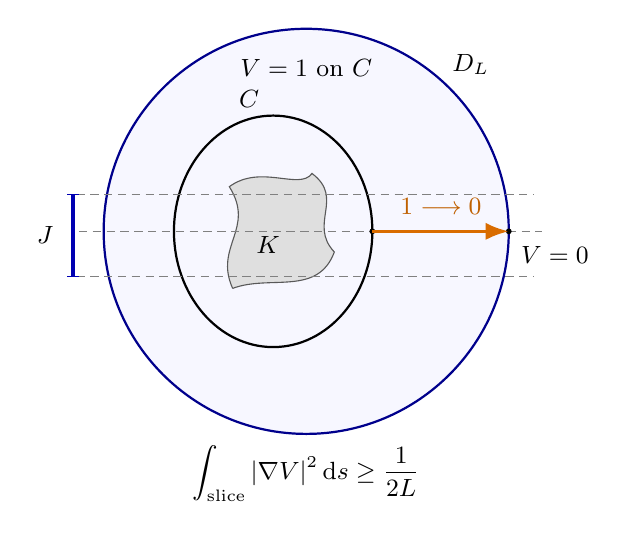
\begin{tikzpicture}[x=1.05cm,y=1.05cm,>=Latex,font=\small]
  \fill[blue!3] (0,0) circle (2.45);
  \draw[blue!55!black,thick] (0,0) circle (2.45);
  \node[anchor=south west] at (1.65,1.78) {$D_L$};
  \draw[thick] (-.40,0) ellipse (1.20 and 1.40);
  \node at (-.69,1.60) {$C$};
  \node at (0,1.98) {$V=1$ on $C$};
  \filldraw[fill=gray!25,draw=gray!70!black]
    (-.89,-.69) .. controls (-1.12,-.18) and (-.61,.03) .. (-.93,.54)
    .. controls (-.55,.82) and (-.08,.49) .. (.07,.70)
    .. controls (.47,.40) and (.02,.09) .. (.34,-.25)
    .. controls (.14,-.79) and (-.44,-.52) .. (-.89,-.69);
  \node at (-.46,-.17) {$K$};
  \draw[gray,densely dashed] (-2.78,-.55) -- (2.75,-.55);
  \draw[gray,densely dashed] (-2.78,.45) -- (2.75,.45);
  \draw[very thick,blue!70!black] (-2.82,-.55) -- (-2.82,.45);
  \draw[blue!70!black] (-2.89,-.55)--(-2.75,-.55);
  \draw[blue!70!black] (-2.89,.45)--(-2.75,.45);
  \node[anchor=east] at (-2.94,-.05) {$J$};
  \draw[gray,densely dashed] (-2.75,0) -- (2.85,0);
  \fill (.80,0) circle (.035);
  \fill (2.45,0) circle (.035);
  \draw[->,very thick,orange!85!black] (.80,0) -- (2.45,0);
  \node[above,orange!75!black] at (1.63,.09) {$1\longrightarrow0$};
  \node[anchor=north west] at (2.48,-.06) {$V=0$};
  \node[align=center] at (0,-2.93)
    {$\displaystyle \int_{\text{slice}}|\nabla V|^2\,\dd s
       \ge \frac{1}{2L}$};
\end{tikzpicture}
\caption{A fixed interval $J$ in a projection of a nondegenerate
component $K$ forces a uniform energy cost. Each corresponding line
meets the inner contour $C$, where the barrier is one, and then reaches
zero within a segment of length at most $2L$. Integrating over $J$
contradicts arbitrarily small barrier energy.
Here $V=V_{n,k}$ and $C=h_n(\gamma_{k,l})$.}
\label{fig:line-payment}
\end{figure}


For definiteness suppose $J$ is the vertical projection interval.
Every horizontal line at a height in $J$ meets the inner image contour, where
$V_{n,k}=1$.  On almost every such line, the Sobolev restriction is
absolutely continuous and agrees with the continuous restriction.
It takes value zero at the left and right ends of the segment with
horizontal coordinates $-L$ and $L$.  Cauchy--Schwarz, followed by
integration over $J$, gives
\begin{equation}\label{eq:line-payment-sobolev}
 \int_\C|\nabla V_{n,k}|^2
 \ge\frac{|J|}{2L}>0.
\end{equation}
The argument only uses the value one on the contour, as illustrated
in Figure~\ref{fig:line-payment}.  Choose $k$ so large that
$k^{-2}<|J|/(2L)$, and then choose $n$ sufficiently late for that
saved contour.  Equations~\eqref{eq:vanishing-barrier-energy}
and~\eqref{eq:line-payment-sobolev} contradict each other.

All limit components are therefore singletons.
Lemma~\ref{lem:ends} now extends $h$ to an orientation-preserving
homeomorphism of the sphere.  Removability of $B$ makes it a M\"obius
map; the normalization $h(z)=z+O(1/z)$ makes it the identity.

Let $A_n$ denote the globally continued first test of the model $h_n$.
Its values on holes are the source endpoint values, and its gradient
vanishes there.  Consequently
\[
 \|A_n\|_\infty\le\|u\|_\infty+1,\qquad
 \|\nabla A_n\|_{2,\Chat}
   =\|\nabla a_n\|_{2,G}\le\|\nabla u\|_{2,G}+1.
\]
Take a weakly convergent subsequence in $W^{1,2}(\Chat)$.  Since
$h_n\to\id$ locally uniformly on $G$, inverse convergence and
\eqref{eq:first-test-control} give $A_n\to u_\epsilon$ locally
uniformly on $G$.  Thus the weak limit equals $u_\epsilon$ there.
Lemma~\ref{lem:null-area} gives $|B|=0$, so the equality holds almost
everywhere on the sphere.  This proves global Sobolev membership of
$u_\epsilon$, with a bound independent of $\epsilon$.  Finally let
$\epsilon\downarrow0$ and use uniform convergence to $u$ and weak
Sobolev compactness once more.  This proves the theorem.
\end{proof}

\section{Null projections of the common point traces}
\label{sec:traces}

We now apply Theorem~\ref{thm:dust-sobolev} to a conformal equivalence
between circle domains.  The scalar functions used below are arranged to
be continuous even when a point component corresponds to a disk.

We first record a packing estimate closely related to
\cite[Lemma~2.1]{Ntalampekos2023}.  We include its short proof from the
Hardy--Littlewood Maximal Theorem \cite{Stein1970}.
\begin{lemma}[Ball synthesis]\label{lem:ball-synthesis}
Let $B_j\subset\R^2$ be balls of radii $d_j>0$.  Suppose there are
pairwise disjoint measurable sets $E_j\subset B_j$ with
$|E_j|\geq c d_j^2$, where $c>0$ is fixed.  For nonnegative
$(a_j)\in\ell^2$,
\[
 \left\|\sum_j\frac{a_j}{d_j}{\bf1}_{B_j}\right\|_{L^2(\R^2)}
 \leq C_c\left(\sum_j a_j^2\right)^{1/2}.
\]
\end{lemma}
\begin{proof}
Let $g\geq0$ belong to $L^2$, and let $Mg$ be its centered maximal
function.  For every $x\in B_j$, the average of $g$ on $B_j$ is at
most $4Mg(x)$, since $B_j\subset B(x,2d_j)$.  Consequently
\begin{align*}
 \int g\sum_j\frac{a_j}{d_j}{\bf1}_{B_j}
 &\leq 4\pi\sum_j a_jd_j\inf_{E_j}Mg\\
 &\leq C_c\left(\sum_j a_j^2\right)^{1/2}
       \left(\sum_j\int_{E_j}(Mg)^2\right)^{1/2}
 \leq C_c\|(a_j)\|_{\ell^2}\|g\|_2.
\end{align*}
Here the last inequality uses disjointness and the $L^2$ Maximal
Theorem.  Duality proves the assertion for finite sums, and monotone
convergence proves it for countable sums.
\end{proof}

For $e\in\{1,i\}$ write $\pi_e(w)=\Re(\overline e w)$.
\begin{proposition}[Common point traces]\label{prop:trace-null}
Let $\Omega,\Omega'$ be circle domains containing infinity, and let
$f:\Omega\to\Omega'$ be a conformal equivalence with $f(\infty)=\infty$.
Suppose $\partial\Omega$ is conformally removable.  Let $C$ be the set
of point components of $\Chat\setminus\Omega$ whose corresponding
components in $\Chat\setminus\Omega'$ are also points, and denote their
positions by $f_*(x)$, $x\in C$.  For each $e\in\{1,i\}$ and almost
every line $\ell$ parallel to $e$,
\[
 \bigl|\{\pi_e(f_*(x)):x\in C\cap\ell\}\bigr|=0.
\]
Here and below $|\cdot|$ for a subset of a line denotes Lebesgue length.
\end{proposition}
\begin{proof}
We fix $e$ throughout.  All complementary components on either side
lie in bounded planar regions.  Index those pairs $(K_j,K'_j)$ for
which at least one component is a disk of positive radius.  The index
set is finite or countable, since disjoint positive-radius disks have
disjoint nonempty interiors.  Write
\[
 K_j=\overline B(a_j,r_j),\qquad
 K'_j=\overline B(a'_j,s_j),
\]
allowing radius zero, and set $\beta_j=\pi_e(a'_j)$.  Disjointness and
boundedness give
\begin{equation}\label{eq:trace-radius-sums}
 \sum_jr_j^2<\infty,\qquad \sum_js_j^2<\infty.
\end{equation}
The other components are precisely the common points in $C$.

\smallskip\noindent
\emph{Scalar data and shrinking neighborhoods.}
Choose a smooth planar cutoff $\chi$, equal to one on a sufficiently
large disk containing the source complement and all the neighborhoods
introduced below, with its transition region compactly contained in
$\Omega$.  On $\Omega$ put
\[
 b=\chi\,\pi_e(f),
\]
and extend $b$ by $\beta_j$ on $K_j$, by $\pi_e(f_*(x))$ on $C$, and
by zero at infinity.  This is bounded.  Indeed, $f(\infty)=\infty$
implies that the image of a bounded source region is bounded.  The
area formula for the univalent map $f$ then shows that $b$ has finite
Dirichlet energy on $\Omega$; the cutoff-derivative term is supported
in a compact subset of $\Omega$.

Although $b$ need not be continuous at $K_j$, it is continuous at
every common point.  Moreover, the cluster values near $K_j$ lie in
$[\beta_j-s_j,\beta_j+s_j]$.  These statements include approaches
through other complementary components and follow from the
upper-semicontinuous correspondence in Lemma~\ref{lem:ends}.

Choose $\varepsilon_j>0$ tending to zero with
$\sum_j\varepsilon_j^2<\infty$, and put
\[
 I_j=(\beta_j-s_j-\varepsilon_j,\,
          \beta_j+s_j+\varepsilon_j),\qquad l_j=|I_j|.
\]
Thus $(l_j)\in\ell^2$.  Fix $A$ so large that all these intervals and
all values of $b$ lie in $(-A,A)$.  Choose positive $\Delta_j$ with
\begin{equation}\label{eq:trace-small-radii}
 \sum_{i>j}\Delta_i^2<\frac12\Delta_j^2;
\end{equation}
for example, a sufficiently small multiple of $2^{-j}$ suffices.
For each integer $m\geq1$, define the balloons
\[
 B_{j,m}=B(a_j,d_{j,m}),\qquad
 d_{j,m}=
 \begin{cases}
  (1+1/m)r_j,&r_j>0,\\
  \Delta_j/m,&r_j=0.
 \end{cases}
\]
These balls are all in one bounded region, and decrease to $K_j$ as
$m\to\infty$.  Choose radial Lipschitz functions
$0\leq\lambda_{j,m}\leq1$ that vanish on an open neighborhood of
$K_j$, equal one outside $B_{j,m}$, and satisfy
\begin{equation}\label{eq:trace-cutoff-gradient}
 |\nabla\lambda_{j,m}|
 \leq\frac{C_m}{d_{j,m}}{\bf1}_{B_{j,m}}
 \quad\hbox{almost everywhere}.
\end{equation}
One may take $C_m=2(m+1)$, interpolating radially between
$(1+1/(2m))r_j$ and $(1+1/m)r_j$ when $r_j>0$, and between
$d_{j,m}/2$ and $d_{j,m}$ otherwise.

For the moment fix $m$ and suppress it from the notation.  We will
transform the scalar value $b(z)$ before applying Sobolev extension.
Near $K_j$ the transformation should be constant on $I_j$, so it does
not distinguish the possible cluster values of $b$.  The cutoff
$\lambda_j$ imposes no restriction outside $B_j$.  Taking the
infimum of the cutoffs whose intervals contain a given scalar value
enforces these requirements simultaneously, including where the
intervals and neighborhoods overlap.  Integrating in the scalar
variable makes the spatial cost proportional to $l_j$, as the
estimate below will show.  Define
\begin{equation}\label{eq:trace-mask}
 L(z,t)=\inf_{j:\,t\in I_j}\lambda_j(z),\qquad
 F(z,t)=\int_{-A}^{t}L(z,s)\,\dd s,\qquad U(z)=F(z,b(z)),
\end{equation}
with the empty infimum equal to one.  We shall prove that $U$ is
continuous and belongs to $W^{1,2}(\Chat)$.

\smallskip\noindent
\emph{An energy density.}
Set
\begin{equation}\label{eq:trace-density}
 P=C_m\sum_j\frac{l_j}{d_j}{\bf1}_{B_j}.
\end{equation}
This belongs to $L^2(\C)$.  For the positive-radius sublist, the
interiors of the original disks $K_j$ are disjoint subsets of $B_j$
of area at least $\pi d_j^2/4$, so Lemma~\ref{lem:ball-synthesis}
applies.  For the zero-radius sublist use instead
\[
 E_j=B_j\setminus\bigcup_{i>j,\,r_i=0}B_i.
\]
These sets are pairwise disjoint: if $i<j$, then $E_i$ excludes
$B_j\supset E_j$.  Since all zero-radius balloons in this system
use the same factor $1/m$, \eqref{eq:trace-small-radii} gives
\[
 |E_j|\geq\pi d_j^2-\pi\sum_{i>j,\,r_i=0}d_i^2
 \geq\tfrac12\pi d_j^2.
\]
Apply Lemma~\ref{lem:ball-synthesis} separately to this sublist and
then add the two $L^2$ bounds.  Overlap between the two sublists is
irrelevant.

\smallskip\noindent
\emph{Continuity of the masks.}
We spell out the accumulation issue.  For fixed $m$, $d_j\to0$.
If distinct balloon supports accumulate at a common point $x$, their
centers and source components approach $x$.  By Lemma~\ref{lem:ends}
their target components approach $\{f_*(x)\}$; as
$\varepsilon_j\to0$, the corresponding intervals $I_j$ approach
the scalar $b(x)$.  Consequently, given $\delta>0$, there are a
neighborhood $V$ of $x$ and a finite initial list such that every
remaining balloon meeting $V$ has its interval in
$(b(x)-\delta,b(x)+\delta)$.  The finite-mask version of $F$ differs
from $F$ by at most $2\delta$ on $V$, uniformly in the upper endpoint.
Since the finite-mask version is continuous in its two variables and
$b$ is continuous at $x$, $U$ is continuous there.

For an indexed component $K_j$, choose a neighborhood $V_j$ of the
entire closed component on which $\lambda_j=0$ and $b\in I_j$.
This is possible because $I_j$ has a positive margin around all its
cluster values.  On $V_j$ the upper endpoint in
\eqref{eq:trace-mask} may be replaced by the fixed value $\beta_j$.
All sufficiently late intervals of balloons meeting a sufficiently
small neighborhood of $K_j$ lie in $I_j$.  To verify the uniformity
of this assertion, a failure would give $i_\nu\to\infty$ and
$z_\nu\in B_{i_\nu}$ with $\dist(z_\nu,K_j)\to0$, but
$I_{i_\nu}\not\subset I_j$.  Passing to a subsequence gives
$z_\nu\to x\in K_j$; the shrinking radii imply
$K_{i_\nu}\to\{x\}$.  Component correspondence puts their target
components arbitrarily close to $K'_j$, and the vanishing extra
margins then force $I_{i_\nu}\subset I_j$, a contradiction.
These late intervals have no effect on $L$ near $K_j$: there
$\lambda_j=0$, so $L(z,t)=0$ for $t\in I_j$.  Thus near $K_j$ the fixed-endpoint expression
is a finite continuous mask.  This proves continuity there, including
when $r_j=0<s_j$.

In $\Omega$ the cutoffs are locally finite, and near infinity they
are all one.  Hence the remaining continuity assertions are
immediate, with $U=A$ near infinity.

\smallskip\noindent
\emph{Sobolev regularity and the residual dust.}
Let $L_N,F_N,U_N$ denote the masks using just the first $N$ indices.
For $t\in[-A,A]$ and any $x,y$,
\begin{equation}\label{eq:trace-finite-variation}
 |F_N(x,t)-F_N(y,t)|
 \leq\sum_{j\leq N}l_j|\lambda_j(x)-\lambda_j(y)|.
\end{equation}
This follows from the elementary difference bound for finite minima,
integrated over the intervals on which a cutoff can occur.  Changing
the upper endpoint costs at most its change, since $0\leq L_N\leq1$.
It follows that $U_N$ has gradient bounded by $|\nabla b|+P$ locally
in $\Omega$.  On $V_j$, once $N\geq j$, its endpoint can be fixed
at $\beta_j$, and its gradient is bounded by $P$.

Bounded pointwise convergence of the finite masks gives local strong
$L^2$ convergence.  Weak Sobolev compactness therefore proves that
$U$ is locally Sobolev on
\[
 O=\Omega\cup\bigcup_jV_j,
\]
with the same gradient bounds.  These yield the finite total energy
estimate
\begin{equation}\label{eq:trace-off-dust-energy}
 \int_O|\nabla U|^2
 \leq2\int_\Omega|\nabla b|^2+2\int_\C P^2<\infty.
\end{equation}
Here the open union is integrated once; no multiplicity is introduced
by overlapping neighborhoods.

The residual set $B_* = \Chat\setminus O$ is compact and bounded,
and consists only of common point components.  Every connected
subset of $B_*$ lies in one component of
$\Chat\setminus\Omega$, hence is a singleton.  Thus $B_*$ is
totally disconnected.  Moreover $B_*\subset\partial\Omega$, and
so it is conformally removable by inclusion.  Theorem~\ref{thm:dust-sobolev},
applied to the continuous bounded function $U$ and
\eqref{eq:trace-off-dust-energy}, proves $U\in W^{1,2}(\Chat)$.
If $B_*$ is empty, this conclusion already follows from the local
Sobolev statement and the energy bound.  We have established the
conclusion for every mask system $m$; denote its function and density
by $U_m,P_m$.

\smallskip\noindent
\emph{A typical line and compression.}
Choose a line $\ell$ parallel to $e$ on which all $U_m$ are locally
absolutely continuous and all $P_m$ are locally integrable.
Almost every such line has these properties, since there are only
countably many systems.  We also require
\begin{equation}\label{eq:trace-line-tail}
 |\partial\Omega\cap\ell|=0,
 \qquad
 \sum_{j:\,B_{j,1}\cap\ell\ne\varnothing}l_j<\infty.
\end{equation}
The first condition holds on almost every line by
Lemma~\ref{lem:null-area} and Fubini.  For the second, write $\ell_\tau$
for the parallel line with transverse coordinate $\tau$.  Tonelli gives
\[
 \int_\R\sum_{j:\,B_{j,1}\cap\ell_\tau\ne\varnothing}l_j\,\dd\tau
 =2\sum_jl_jd_{j,1}<\infty,
\]
by Cauchy--Schwarz and \eqref{eq:trace-radius-sums}--\eqref{eq:trace-small-radii}.
Fix a line satisfying all these conditions.

For $N\geq1$ let
\[
 I^{(N)}=\bigcup_{\substack{j>N\\B_{j,1}\cap\ell\ne\varnothing}}I_j,
 \qquad
 H_N(t)=\int_{-A}^{t}{\bf1}_{\R\setminus I^{(N)}}(s)\,\dd s.
\]
Equation~\eqref{eq:trace-line-tail} implies $|I^{(N)}|\to0$.
For any $x\in C\cap\ell$, the distance from $x$ to each of the
first $N$ closed components is positive.  Some system $m$ therefore
has an open line neighborhood $J$ of $x$ missing its first $N$
balloons.  On $J$, every active cutoff belongs to the tail appearing
in $I^{(N)}$, and hence
\[
 L_m(z,t)\geq{\bf1}_{\R\setminus I^{(N)}}(t).
\]
The fixed-endpoint variation estimate extends to the infinite mask:
for any segment $[x,y]\subset\ell$ and fixed $t\in[-A,A]$,
\begin{equation}\label{eq:trace-segment-variation}
 |F_m(x,t)-F_m(y,t)|\leq\int_{[x,y]}P_m\,\dd s.
\end{equation}
Indeed \eqref{eq:trace-cutoff-gradient} and
\eqref{eq:trace-finite-variation} give this for finite masks, and
dominated convergence in the integration variable gives the limit.
The estimate uses only the globally Lipschitz cutoffs, so it remains
valid when the segment crosses indexed components where $b$ is
discontinuous.

If $x,y\in C\cap J$, compare the two upper endpoints at one fixed
location, and then use \eqref{eq:trace-segment-variation}.  The
nonnegative-integrand inequality above gives
\begin{align}
 |H_N(b(x))-H_N(b(y))|
 &\leq |U_m(x)-U_m(y)|+\int_{[x,y]}P_m\,\dd s\notag\\
 &\leq\int_{[x,y]}(|U_m'|+P_m)\,\dd s.
 \label{eq:trace-compression-bound}
\end{align}
For example, when $b(x)\leq b(y)$, first bound the compressed
increment by $F_m(x,b(y))-F_m(x,b(x))$ and then replace
$F_m(x,b(y))$ by $F_m(y,b(y))$.  The other order is identical.

The set $C\cap J$ has length zero.  A general elementary consequence
of \eqref{eq:trace-compression-bound} is therefore
\[
 |H_N(b(C\cap J))|=0.
\]
To see this with outer length, work first in a compact subinterval
of $J$.  Cover its null set of common points by an open set on which
the integral of $|U_m'|+P_m$ is arbitrarily small.  On each component
interval, \eqref{eq:trace-compression-bound} bounds the diameter of
the image of the common points by that integral.  Summing gives
arbitrarily small interval covers of the image.  A countable
exhaustion proves the assertion on $J$.

We recover the uncompressed values by the one-dimensional area
formula.  The common-point set is Borel, since it is the compact
complement with the countable union of the indexed closed components
removed.  Its trace map is continuous in the relative topology.
Thus $b(C\cap J)$ is analytic and Lebesgue measurable.  Put
$S=b(C\cap J)\setminus I^{(N)}$.  The nondecreasing Lipschitz
function $H_N$ has derivative one almost everywhere outside
$I^{(N)}$, and hence
\[
 |S|=\int_S|H_N'|
 =\int_\R\#\{t\in S:H_N(t)=u\}\,\dd u=0.
\]
The last integrand is supported on the null set
$H_N(b(C\cap J))$.  This reasoning allows both noninjectivity of
$H_N$ and its null set of derivative exceptions.

For fixed $N$, countably many of the neighborhoods $J$ suffice to
cover $C\cap\ell$, by the countable base of the line.  It follows
that $b(C\cap\ell)\setminus I^{(N)}$ is null.  Finally
$|I^{(N)}|\to0$, so $|b(C\cap\ell)|=0$.  Since $b(x)=\pi_e(f_*(x))$
on common points, this is the required conclusion.  Empty or finite
indexed lists are included by interpreting the corresponding sums
and tails in the evident way.
\end{proof}

\section{The length--area argument}\label{sec:rigidity}

The trace statement now supplies the line estimates needed for a flux
lower bound.  Comparing that bound with the source and target area
bounds will force the normalized conformal map to have derivative of
unit modulus and corresponding disks to have equal radii.

\begin{proof}[Proof of Theorem~\ref{thm:main}]
If $\Omega=\Chat$, its conformal image is also the sphere, by
compactness, and its automorphisms are M\"obius transformations.
Assume henceforth that the complement is nonempty.  Apply separate
M\"obius changes in source and target to move a domain point and its
image to infinity.  A further target affine change gives
\begin{equation}\label{eq:rigidity-normalization}
 f(z)=z+\sum_{n\ge1}\alpha_nz^{-n}
 \quad\text{near infinity}.
\end{equation}
These changes preserve circle domains and conformal removability.
All complementary components are now bounded Euclidean disks or
points.  Their correspondence is supplied by Lemma~\ref{lem:ends}.

Index by $j$ precisely those corresponding pairs for which at least
one component is nondegenerate.  Write
\[
 K_j=\overline D(a_j,r_j),\qquad
 K'_j=\overline D(b_j,s_j),
\]
allowing a zero radius to mean a singleton.  The index set is finite
or countable, and
\begin{equation}\label{eq:radius-summability}
 \sum_jr_j^2<\infty,\qquad \sum_js_j^2<\infty,\qquad
 \sum_jr_js_j<\infty.
\end{equation}
Indeed the positive-radius disks on each side have disjoint interiors
in a bounded region, and the last assertion follows by
Cauchy--Schwarz.  All other complementary components are common
points: both the source and target component are singletons.
Let $\tau$ denote their correspondence.

Choose $R$ strictly larger than a radius containing the source
complement.  Define a vector field $F$ on $\overline D_R$ by using
$f$ in $\Omega$, the center $b_j$ on $K_j$, and $\tau(p)$ at every
common point $p$.  This is a bounded measurable field.  Boundedness
follows from Lemma~\ref{lem:ends}, or from the bounded side of the
image outer contour.  Measurability follows since there are
countably many indexed closed components, the common-point set is
Borel, and its singleton trace map is continuous relative to that
set.  No continuity of $F$ at an indexed component is asserted.

\paragraph{A slice estimate.}
Remove disjoint slightly enlarged concentric disks around the first
$N$ indexed source components, using a positive enlargement also when
$r_j=0$.  Denote the remaining round region by $A_N$.  The sizes of
the enlargements will tend to zero with $N$ fixed.

Consider a closed component segment $J=[x,y]$ of an axial slice of
$A_N$, directed toward increasing coordinate.  At domain points use
the projected value of $f$; at a complementary component use the
entire projection interval of its corresponding target component.
These fibers are compact intervals in a fixed bounded interval, and
their relation has closed graph by Lemma~\ref{lem:ends}.  Their union
over $J$ is connected.  To verify this directly, a missing value $t$
between two attained values would place each fiber wholly below or
wholly above $t$.  Upper semicontinuity makes these two classes open
in $J$, giving a separation of the segment.

Consequently all values between the selected endpoint values are
covered by the projected images of domain arcs, common-point traces,
and the full intervals of met indexed components.  By
Proposition~\ref{prop:trace-null}, the common traces have length zero
on almost every such line.  The countably many domain arcs have
total projected-image length at most the integral of $|f'|$ over
them.  Each met indexed component contributes at most $2s_j$.
Writing $F_{\rm ax}$ for the coordinate along the slice, we obtain
\begin{equation}\label{eq:slice-estimate}
 F_{\rm ax}(y)-F_{\rm ax}(x)
 \le \int_{J\cap\Omega}|f'|\,\dd s
       +\sum_{\substack{j>N\\K_j\cap J\ne\varnothing}}2s_j
\end{equation}
for almost every line in either direction.  In fact the same argument
bounds the absolute endpoint difference.  Endpoints on an enlarged
circle use the same field $F$ for both slicing directions.

\paragraph{Multiplicity of the tail terms.}
For fixed $N$ the enlargements can be chosen so that each remaining
positive-radius source component meets at most one enlarged disk.
For $N\ge2$, let $\delta>0$ be the minimum separation of the first
$N$ source components.  Make their enlargements small enough to
retain gaps greater than $\delta/2$.  A remaining disk of diameter
less than $\delta/2$ cannot meet two of them.  Only finitely many
remaining disks have larger diameter, and their positive distances
from the first $N$ components permit further shrinking of the
enlargements so that these finitely many disks meet none.  This
argument includes point components among the first $N$.  For $N=1$
there is nothing to prove, and for $N=0$ nothing is removed.

A line meets a remaining disk in an interval; deleting at most one
enlarged-disk interval leaves at most two retained pieces.  Thus its
cost in \eqref{eq:slice-estimate} is counted at most twice.  Integrating
transversely gives at most $8r_js_j$ per direction and at most
$16r_js_j$ for both directions.  Indexed source point components are
missed by almost every axial line, even when their target components
are disks.  All exceptional indexed point lines form a countable set.
The tail estimates are integrable by \eqref{eq:radius-summability}.

\paragraph{Flux.}
Integrating \eqref{eq:slice-estimate} over horizontal and vertical
lines gives the flux through the outer circle minus the flux through
the enlarged inner circles.  This is the elementary projection
formula for arclength on a circle: the transverse projection Jacobians
are $|n_X|$ for horizontal slices and $|n_Y|$ for vertical slices.
It applies to bounded measurable boundary values.  The normal on an inner circle is taken outward
from its removed disk.  The two domain integrals are bounded by
$2\int_{\Omega\cap D_R}|f'|\,\dd A$.

On the outer circle $F=f$, and
\eqref{eq:rigidity-normalization} gives exactly
\begin{equation}\label{eq:outer-flux}
 \int_{\partial D_R}F\cdot n\,\dd s
 =\operatorname{Re}\int_0^{2\pi}
     f(Re^{it})e^{-it}R\,\dd t
 =2\pi R^2.
\end{equation}
On the enlarged circle about $K_j$, subtract the constant target
center $b_j$, whose flux is zero.  As its radius decreases to $r_j$,
Lemma~\ref{lem:ends} puts all its assigned values within distance
$s_j+o(1)$ of $b_j$, uniformly along the circle.  Hence its inner
outward flux $I_j$ satisfies
\begin{equation}\label{eq:inner-flux}
 \limsup I_j\le2\pi r_js_j.
\end{equation}
When $r_j=0$ the circle length tends to zero; when $s_j=0$ the target
displacement tends to zero.  Thus both types of mismatch are covered.

Moving the inner fluxes to the right and letting the finitely many
enlargements shrink, while retaining the preceding multiplicity
property, gives
\[
 2\pi R^2
 \le 2\int_{\Omega\cap D_R}|f'|\,\dd A
    +2\pi\sum_{j\le N}r_js_j
    +16\sum_{j>N}r_js_j.
\]
Let $N$ exhaust the indexed components.  In the finite or empty case
the corresponding terminal sum is already zero.  We conclude that
\begin{equation}\label{eq:limiting-flux}
 2\pi R^2\le2\int_{\Omega\cap D_R}|f'|\,\dd A
                      +2\pi\sum_jr_js_j.
\end{equation}

\paragraph{Area and equality.}
The source domain portion and the interiors of its complementary
disks are disjoint subsets of $D_R$, so
\begin{equation}\label{eq:source-area}
 \int_{\Omega\cap D_R}1\,\dd A+\pi\sum_jr_j^2\le\pi R^2.
\end{equation}
The image of $\partial D_R$ is a Jordan contour.  Its bounded side
contains $f(\Omega\cap D_R)$ and all target complementary components:
the compact exterior source disk is mapped homeomorphically onto the
closed Jordan side containing infinity.  Indeed its interior is mapped
openly, its boundary is the image contour, and compactness makes its
image closed in that side; connectedness then identifies the entire
side.  These pieces are disjoint.  By the Laurent
area formula its enclosed area is
\[
 \pi R^2-\pi\sum_{n\ge1}n|\alpha_n|^2R^{-2n}\le\pi R^2.
\]
Conformal change of variables therefore gives
\begin{equation}\label{eq:target-area}
 \int_{\Omega\cap D_R}|f'|^2\,\dd A
       +\pi\sum_js_j^2\le\pi R^2.
\end{equation}
No area-zero assertion about the target dust is needed: any area in
its uncountably many singleton components is simply omitted from
the left side of this inequality.

Adding \eqref{eq:source-area} and \eqref{eq:target-area}, then using
\eqref{eq:limiting-flux}, yields
\begin{equation}\label{eq:nonnegative-rigidity}
 \boxed{\displaystyle
 \int_{\Omega\cap D_R}(|f'|-1)^2\,\dd A
       +\pi\sum_j(r_j-s_j)^2\le0.}
\end{equation}
Both terms are nonnegative.  Continuity of the integrand shows that
$|f'|=1$ throughout the nonempty open set $\Omega\cap D_R$.  On any
disk compactly contained in this set, the Open Mapping Theorem makes
$f'$ constant, so $f(z)=\lambda z+c$ there.  The meromorphic Identity
Theorem on the connected domain $\Omega$ gives this equality
everywhere in $\Omega$.  Finally
\eqref{eq:rigidity-normalization} forces $\lambda=1$ and $c=0$.
Undoing the source and target changes of coordinates proves that the
original equivalence is the restriction of a M\"obius transformation.
\end{proof}

\bibliographystyle{plain}
\bibliography{references}
\end{document}
